\section*{Problem 1}

\subsection*{1.1}
Expand the scalar function and differentiate with respect to an arbitrary coordinate $w_k$:
\begin{align*}
g(\mathbf{w})&=\sum_{i=1}^{n}b_iw_i+\frac12\sum_{i=1}^{n}\sum_{j=1}^{n}A_{ij}w_iw_j\\
\frac{\partial g}{\partial w_k}
&=b_k+\frac12\sum_{j=1}^{n}A_{kj}w_j
       +\frac12\sum_{i=1}^{n}A_{ik}w_i\\
\end{align*}
Since A is a symmetric matrix, so: $A_{ik}=A_{ki}$\\
\\
And we rename the index $i$ to $j$
Thus:
\begin{align*}
\frac{\partial g}{\partial w_k}
&=b_k+\sum_{j=1}^{n}A_{kj}w_j\\
&=(\mathbf{b}+A\mathbf{w})_k
\end{align*}
Thus:\\
\begin{align*}
{\nabla_{\mathbf{w}}g(\mathbf{w})=\mathbf{b}+A\mathbf{w}}
\end{align*}

\subsection*{1.2}
Every column of $\mathbf{x}\mathbf{x}^{\top}$ is a scalar multiple of $\mathbf{x}$, which is in the form of $x_j\mathbf{x}$, so its column space is contained in $\operatorname{span}\{\mathbf{x}\}$ and its rank is at most 1. Since $\mathbf{x}\ne\mathbf{0}$, some $x_j\ne0$, so column $j$ equals the nonzero vector $x_j\mathbf{x}$.\\
Thus:\\
\begin{align*}
\operatorname{rank}(\mathbf{x}\mathbf{x}^{\top})=1
\end{align*}

\subsection*{1.3}
Since $A\in\mathbb{R}^{m\times n}$ and $B\in\mathbb{R}^{n\times m}$,\\\\
Thus, $AB\in\mathbb{R}^{m\times m}$, $BA\in\mathbb{R}^{n\times n}$, and:\\
\begin{align*}
\operatorname{tr}(AB)
=\sum_{i=1}^{m}(AB)_{ii}\\
\operatorname{tr}(BA)
=\sum_{j=1}^{n}(BA)_{jj}
\end{align*}
Since: 
\begin{align*}
(AB)_{ii}
=\sum_{j=1}^{n}A_{ij}B_{ji}\\
(BA)_{jj}
=\sum_{i=1}^{m}B_{ji}A_{ij}
\end{align*}
Thus: 
\begin{align*}
\operatorname{tr}(AB)
=\sum_{i=1}^{m}\sum_{j=1}^{n}A_{ij}B_{ji}\\
\operatorname{tr}(BA)
=\sum_{j=1}^{n}\sum_{i=1}^{m}B_{ji}A_{ij}
\end{align*}
Thus:
\begin{align*}
\operatorname{tr}(AB)
=\sum_{i=1}^{m}\sum_{j=1}^{n}A_{ij}B_{ji}
=\operatorname{tr}(BA)
\end{align*}

\subsection*{1.4}
The matrix $A=\left(\begin{smallmatrix}2&1\\1&2\end{smallmatrix}\right)$ is symmetric. For every $\mathbf{x}=(x_1,x_2)^{\top}\in\mathbb{R}^2$,
\[
\mathbf{x}^{\top}A\mathbf{x}=2x_1^2+2x_1x_2+2x_2^2
=(x_1+x_2)^2+x_1^2+x_2^2\ge0.
\]
Since $\mathbf{x}^{\top}A\mathbf{x}\ge0$,\\\\
Therefore, the expression is positive for every nonzero $\mathbf{x}$, so $A$ is positive definite.

\clearpage
\section*{Problem 2}

\subsection*{2.1: Distribution shift (external validity)}
Because the deployment distribution consists of 2026 social-media posts rather than 2019 movie reviews. And the strong IID test accuracy on the original distribution does not transfer to this new distribution.

\subsection*{2.2: Contamination}
Because the public benchmark questions and answers may entered the model's training data. And its score may reflect on memorization instead of performance on unseen questions.

\subsection*{2.3: Adaptive overfitting}
Because repeatedly selecting among 300 tweaks using the same public test set makes that set part of model selection. The chosen model can exploit that set's sampling noise and have a higher public-test score relative to fresh data from the same source.

\subsection*{2.4: Construct validity}
Because multiple-choice medical licensing exam performance measures a different capability from diagnosing real patients. The exam score alone cannot prove it is ready to diagnose real patients.

\newpage
\section*{Problem 3}

\subsection*{3.1}
Let $Z_1,\ldots,Z_n\in\{0,1\}$ be IID indicators of correct predictions by a fixed model, and let
$A_n=\frac1n\sum_{i=1}^{n}Z_i$ and $\mu=\mathbb{E}[Z_i]$. Hoeffding's inequality gives:
\[
\mathbb{P}(|A_n-\mu|\ge\epsilon)\le 2e^{-2n\epsilon^2}
\]
For failure probability at most $\delta$:
\begin{align*}
2e^{-2n\epsilon^2}\le\delta\\
n\ge\frac{\ln(2/\delta)}{2\epsilon^2}
\end{align*}
A sufficient integer size is therefore:
\begin{align*}
n=\left\lceil\ln(2/\delta)/(2\epsilon^2)\right\rceil
\end{align*}
At $\delta=0.05$, $\ln(2/\delta)=\ln40\approx3.688879454$:
\begin{center}
\begin{tabular}{@{}lrr@{}}
\toprule
Precision $\epsilon$ & Bound before rounding & Sufficient size $n$\\
\midrule
$0.01$ (1 percentage point) & $18{,}444.3973$ & $18{,}445$\\
$0.001$ (0.1 percentage point) & $1{,}844{,}439.7271$ & $1{,}844{,}440$\\
\bottomrule
\end{tabular}
\end{center}
At fixed confidence, $n$ scales as $1/\epsilon^2$. One additional decimal digit of certified precision divides $\epsilon$ by 10 and requires approximately \textbf{100 times as many test examples}. These are sufficient Hoeffding bounds.

\subsection*{3.2(i). Individual 95\% confidence half-widths}
Solving $\delta_j=2e^{-2n_j\epsilon_j^2}$ with $\delta_j=0.05$ gives
$\epsilon_j=\sqrt{\ln40/(2n_j)}$. Thus
\[
\boxed{\epsilon_1\approx0.006073615}\quad(n_1=50{,}000),
\qquad
\boxed{\epsilon_2\approx0.013581015}\quad(n_2=10{,}000).
\]
These half-widths are approximately $0.6074$ and $1.3581$ percentage points, respectively.

\subsection*{3.2(ii)(a). Probability of simultaneous validity}
Let $C_j=[A_j-\epsilon_j,A_j+\epsilon_j]$ and $E_j=\{\mu\notin C_j\}$.
Since $\mathbb{P}(E_j)\le\delta_j$, the union bound gives
\[
\boxed{\mathbb{P}(\text{simultaneous validity fails})
=\mathbb{P}(E_1\cup E_2)
\le\mathbb{P}(E_1)+\mathbb{P}(E_2)
\le\delta_1+\delta_2.}
\]
Both intervals therefore contain $\mu$ with probability at least $1-\delta_1-\delta_2$.
This union-bound argument does not require independence.

\subsection*{3.2(ii)(b). Overlap and the accuracy difference}
If both intervals contain $\mu$, then $\mu\in C_1\cap C_2$, so they overlap.
The triangle inequality also gives
\[
\boxed{|A_1-A_2|\le|A_1-\mu|+|A_2-\mu|\le\epsilon_1+\epsilon_2.}
\]
Here, $\epsilon_1+\epsilon_2\approx0.019654630$, or $1.9655$ percentage points.
The union bound guarantees simultaneous coverage, and hence this difference bound, with probability at least $0.90$.
With the stated independence of the test sets, simultaneous coverage is at least $0.95^2=0.9025$.

\newpage
\section*{Problem 4: Mini-batch gradient noise}
The training data and current parameter $\mathbf{w}$ are fixed. Let $\mathbf{g}_i\in\mathbb{R}^d$ be the gradient of the loss for example $i$, and define
\[
\mathbf{g}=\frac1n\sum_{i=1}^{n}\mathbf{g}_i,
\qquad
\sigma^2=\frac1n\sum_{i=1}^{n}\|\mathbf{g}_i-\mathbf{g}\|^2.
\]
All expectations below are over the sampled indices.

\subsection*{4.1. One uniformly sampled example}
Because $\mathbb{P}(I=i)=1/n$,
\[
\boxed{\mathbb{E}[\mathbf{g}_I]=\sum_{i=1}^{n}\frac1n\mathbf{g}_i=\mathbf{g}},
\qquad
\boxed{\mathbb{E}\!\left[\|\mathbf{g}_I-\mathbf{g}\|^2\right]
=\frac1n\sum_{i=1}^{n}\|\mathbf{g}_i-\mathbf{g}\|^2=\sigma^2}.
\]

\subsection*{4.2. A mini-batch sampled independently with replacement}
For independent uniform indices $I_1,\ldots,I_B$, define
$\widehat{\mathbf{g}}_B=\frac1B\sum_{b=1}^{B}\mathbf{g}_{I_b}$.
By linearity of expectation and the result of part 4.1,
\[
\boxed{\mathbb{E}[\widehat{\mathbf{g}}_B]
=\frac1B\sum_{b=1}^{B}\mathbb{E}[\mathbf{g}_{I_b}]
=\frac1B\sum_{b=1}^{B}\mathbf{g}=\mathbf{g}}.
\]
Define $\mathbf{z}_b=\mathbf{g}_{I_b}-\mathbf{g}$. Then the $\mathbf{z}_b$ are independent, $\mathbb{E}[\mathbf{z}_b]=\mathbf{0}$,
and $\mathbb{E}\|\mathbf{z}_b\|^2=\sigma^2$. For $b\ne c$, independence and zero mean give
\[
\mathbb{E}[\mathbf{z}_b^{\top}\mathbf{z}_c]
=\sum_{k=1}^{d}\mathbb{E}[z_{b,k}z_{c,k}]
=\sum_{k=1}^{d}\mathbb{E}[z_{b,k}]\mathbb{E}[z_{c,k}]=0.
\]
Expanding the squared norm and substituting these identities yields
\begin{align*}
\mathbb{E}\!\left[\|\widehat{\mathbf{g}}_B-\mathbf{g}\|^2\right]
&=\frac1{B^2}\mathbb{E}\!\left[\left\|\sum_{b=1}^{B}\mathbf{z}_b\right\|^2\right]\\
&=\frac1{B^2}\left(
  \sum_{b=1}^{B}\mathbb{E}\|\mathbf{z}_b\|^2
  +2\sum_{1\le b<c\le B}\mathbb{E}[\mathbf{z}_b^{\top}\mathbf{z}_c]
  \right)\\
&=\frac{B\sigma^2+0}{B^2}=\boxed{\frac{\sigma^2}{B}}.
\end{align*}

\clearpage

\section*{Problem 5: Linear Regression}

\subsection*{5.1 Closed-form solution}

The empirical risk is
\[
\widehat R(\mathbf w)
=\frac{1}{2n}\|X\mathbf w-\mathbf y\|_2^2.
\]
Setting its gradient to zero gives the normal equations
\[
X^\top X\mathbf w_{\mathrm{LS}}=X^\top\mathbf y.
\]
The implementation solves these equations using
\texttt{np.linalg.solve(X.T @ X, X.T @ y)}.

\begin{center}
\begin{tabular}{lr}
\toprule
Quantity & Empirical risk \\
\midrule
Training risk of $\mathbf w_{\mathrm{LS}}$ & 0.117523 \\
Training risk of $\mathbf 0$ & 37.6633 \\
Test risk of $\mathbf w_{\mathrm{LS}}$ & 0.139395 \\
\bottomrule
\end{tabular}
\end{center}

The test risk is approximately 0.021873 higher than the training risk,
using the unrounded values. The parameters are chosen to minimize error
on the training sample and can partly fit its noise. This advantage does
not transfer to fresh examples; finite-sample variation also affects the
observed train--test gap.

The training risk, 0.117523, is below the noise floor
$\operatorname{Var}(\varepsilon)/2=0.5^2/2=0.125$.
The noise floor is the minimum population risk for this data-generating
model, rather than a lower bound on a fitted model's training risk.
Fitting some of the realized training noise can reduce the training risk
below 0.125 without eliminating the noise in future observations.

\clearpage
\subsection*{5.2 Gradient descent}

Differentiating the empirical risk gives
\[
\nabla\widehat R(\mathbf w)
=\frac1n\sum_{i=1}^{n}(\mathbf w^\top\mathbf x_i-y_i)\mathbf x_i
=\frac1nX^\top(X\mathbf w-\mathbf y).
\]
The update is
$\mathbf w_{t+1}=\mathbf w_t-\eta\nabla\widehat R(\mathbf w_t)$.
The final risks after 20 updates are:

\begin{center}
\begin{tabular}{rr}
\toprule
Step size $\eta$ & Final training risk \\
\midrule
0.005 & 30.7255 \\
0.5 & 0.117533 \\
1.3 & 384.81 \\
\bottomrule
\end{tabular}
\end{center}

\begin{figure}[H]
\centering
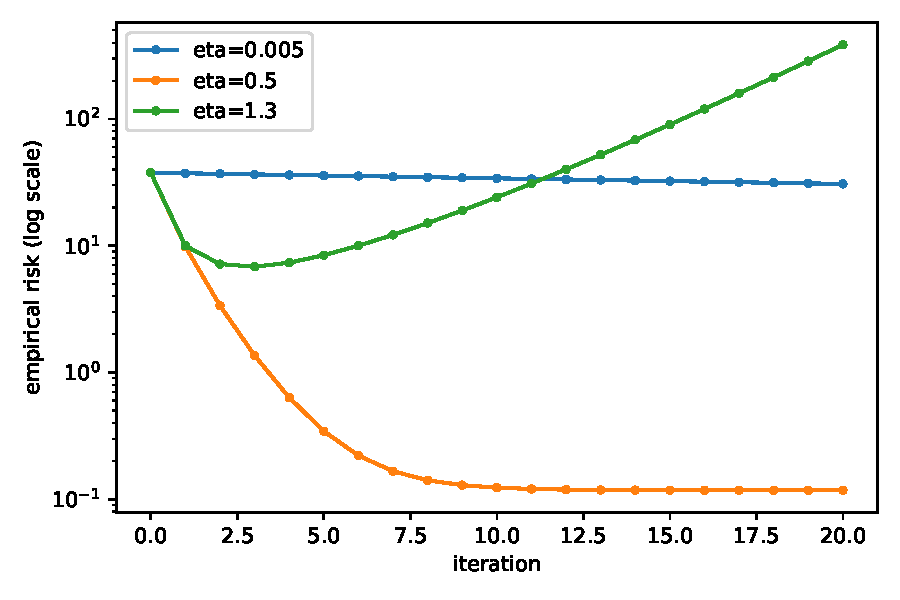
\includegraphics[width=0.72\linewidth]{gd_curves.pdf}
\caption{Full-gradient descent for 20 updates. The vertical axis is logarithmic; iteration zero is the initial risk.}
\label{fig:hw1-p5-gd}
\end{figure}

The step size 0.005 gives slow, stable progress. The step size 0.5 gives
rapid convergence to near the closed-form minimum. The step size 1.3
initially reduces the risk, but then diverges because it is too large.

For this quadratic objective, let $H=X^\top X/n$. The error satisfies
$\mathbf w_{t+1}-\mathbf w_{\mathrm{LS}}
=(I-\eta H)(\mathbf w_t-\mathbf w_{\mathrm{LS}})$.
Convergence for all initial errors requires
$0<\eta<2/\lambda_{\max}(H)$.
For the generated data, $\lambda_{\max}(H)\approx1.721891$, so this upper
limit is approximately 1.161514. The step size 1.3 exceeds it.

The closest result uses $\eta=0.5$. Using unrounded risks, its gap from
the optimum is
\[
0.117532936366-0.117522521822
\approx1.04145\times10^{-5}.
\]

\clearpage
\subsection*{5.3 Stochastic gradient descent}

For the single-example loss
$\ell_i(\mathbf w)=\tfrac12(\mathbf w^\top\mathbf x_i-y_i)^2$,
the gradient is $(\mathbf w^\top\mathbf x_i-y_i)\mathbf x_i$.
Each step draws one index uniformly with replacement and applies
\[
\mathbf w_{t+1}
=\mathbf w_t-\eta(\mathbf w_t^\top\mathbf x_{i_t}-y_{i_t})\mathbf x_{i_t}.
\]
The final risks after 1000 updates are:

\begin{center}
\begin{tabular}{rr}
\toprule
Step size $\eta$ & Final training risk \\
\midrule
0.001 & 5.886 \\
0.01 & 0.23842 \\
0.02 & 94.3621 \\
\bottomrule
\end{tabular}
\end{center}

\begin{figure}[H]
\centering
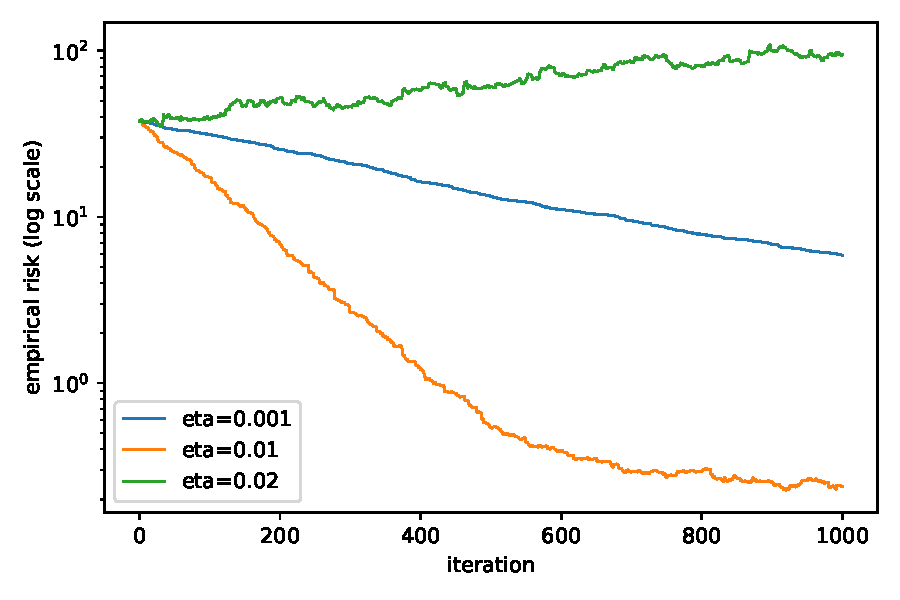
\includegraphics[width=0.64\linewidth]{sgd_curves.pdf}
\caption{SGD for 1000 updates. The vertical axis is logarithmic; every plotted value is the risk on the full training set.}
\label{fig:hw1-p5-sgd}
\end{figure}

\begin{center}
\begin{tabular}{lrr}
\toprule
Update computation per step-size run & GD & SGD \\
\midrule
Individual-example gradients per update & 1000 & 1 \\
Number of updates & 20 & 1000 \\
Total individual-example gradients & 20,000 & 1000 \\
Equivalent passes over the training data & 20 & 1 \\
\bottomrule
\end{tabular}
\end{center}

Sampling with replacement means that one equivalent pass need not visit
every example. These counts exclude monitoring: GD and SGD evaluate the
full-data risk 21 and 1001 times, respectively, including the initial value.

Stable GD uses the full gradient and has smooth decreasing risk. SGD
uses a noisy, unbiased estimate: improving one sampled example may
increase the full risk, producing jagged curves. With a constant step
size, noise generally persists near the optimum. Here, 0.001 progresses
slowly, 0.01 gives the lowest final SGD risk, and 0.02 is unstable.

The best GD risk (0.117533) is below the best SGD risk (0.23842) and
close to the closed-form minimum (0.117523). GD uses 20 times as many
individual-example gradient evaluations per run, so the update budgets
are different.
